\begin{figure*}
  \centering
  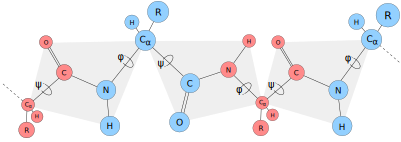
\includegraphics[width=0.75\textwidth]{figures/protein-torsion-angles}
  \label{fig:protein-torsion-angles}
  \caption{}
\end{figure*}

The representation of proteins shown in the structure diagram of
Figure \ref{fig:amino_connect} is suitable for determining the
chemical properties of the molecules, how atoms are arranged and the
bonding between atoms. However, to be able to do calculate on the
precise structure of the proteins we need a more precise
description. That is, we need to include bond lengths, bond angles and
torsional angles into the model.

\section{Backbone geometry}
Torsion angles, phi, psi, (omega)
Bond lengths
Bond angles

% As mentioned in our introduction, the largest variability of the
% protein structure is found in the \textit{torsional} angles between
% the individual $C_\alpha$-atoms \cite{lotan04}. These angles are
% termed $\phi$ and $\psi$ in the literature, Figure
% \ref{fig:protein-torsion-agnles} illustrates their definition.

\section{Side-chain geometry}
Rotamers (evt. calculating bond angles and bond lengths)
